\documentclass[tikz,border=10pt]{standalone}
% Shared look for every TikZ diagram. Load with % Shared look for every TikZ diagram. Load with % Shared look for every TikZ diagram. Load with \input{../../tools/tikz-style.tex}
\usepackage[T1]{fontenc}
\usepackage{lmodern}
\renewcommand{\sfdefault}{lmr}  % diagrams use the same serif as the text
\usetikzlibrary{arrows.meta, positioning, shapes.geometric, calc, fit, backgrounds}
\definecolor{cblue}{HTML}{4C78A8}
\definecolor{corange}{HTML}{F58518}
\definecolor{cgreen}{HTML}{54A24B}
\definecolor{cred}{HTML}{E45756}
\definecolor{cpurple}{HTML}{B279A2}
\definecolor{cgrey}{HTML}{6B6B6B}
\tikzset{
  every picture/.style={font=\sffamily, line width=1.2pt},
  box/.style={draw=#1, fill=#1!12, rounded corners=4pt, align=center, inner sep=7pt, minimum height=1.1cm},
  box/.default=cgrey,
  arrow/.style={-{Stealth[length=3mm]}, draw=cgrey, line width=1.4pt},
  title/.style={font=\sffamily\bfseries\Large},
  note/.style={font=\sffamily\small, text=cgrey, align=center},
}
\AtBeginDocument{\hyphenpenalty=10000 \exhyphenpenalty=10000}

\usepackage[T1]{fontenc}
\usepackage{lmodern}
\renewcommand{\sfdefault}{lmr}  % diagrams use the same serif as the text
\usetikzlibrary{arrows.meta, positioning, shapes.geometric, calc, fit, backgrounds}
\definecolor{cblue}{HTML}{4C78A8}
\definecolor{corange}{HTML}{F58518}
\definecolor{cgreen}{HTML}{54A24B}
\definecolor{cred}{HTML}{E45756}
\definecolor{cpurple}{HTML}{B279A2}
\definecolor{cgrey}{HTML}{6B6B6B}
\tikzset{
  every picture/.style={font=\sffamily, line width=1.2pt},
  box/.style={draw=#1, fill=#1!12, rounded corners=4pt, align=center, inner sep=7pt, minimum height=1.1cm},
  box/.default=cgrey,
  arrow/.style={-{Stealth[length=3mm]}, draw=cgrey, line width=1.4pt},
  title/.style={font=\sffamily\bfseries\Large},
  note/.style={font=\sffamily\small, text=cgrey, align=center},
}
\AtBeginDocument{\hyphenpenalty=10000 \exhyphenpenalty=10000}

\usepackage[T1]{fontenc}
\usepackage{lmodern}
\renewcommand{\sfdefault}{lmr}  % diagrams use the same serif as the text
\usetikzlibrary{arrows.meta, positioning, shapes.geometric, calc, fit, backgrounds}
\definecolor{cblue}{HTML}{4C78A8}
\definecolor{corange}{HTML}{F58518}
\definecolor{cgreen}{HTML}{54A24B}
\definecolor{cred}{HTML}{E45756}
\definecolor{cpurple}{HTML}{B279A2}
\definecolor{cgrey}{HTML}{6B6B6B}
\tikzset{
  every picture/.style={font=\sffamily, line width=1.2pt},
  box/.style={draw=#1, fill=#1!12, rounded corners=4pt, align=center, inner sep=7pt, minimum height=1.1cm},
  box/.default=cgrey,
  arrow/.style={-{Stealth[length=3mm]}, draw=cgrey, line width=1.4pt},
  title/.style={font=\sffamily\bfseries\Large},
  note/.style={font=\sffamily\small, text=cgrey, align=center},
}
\AtBeginDocument{\hyphenpenalty=10000 \exhyphenpenalty=10000}

\begin{document}
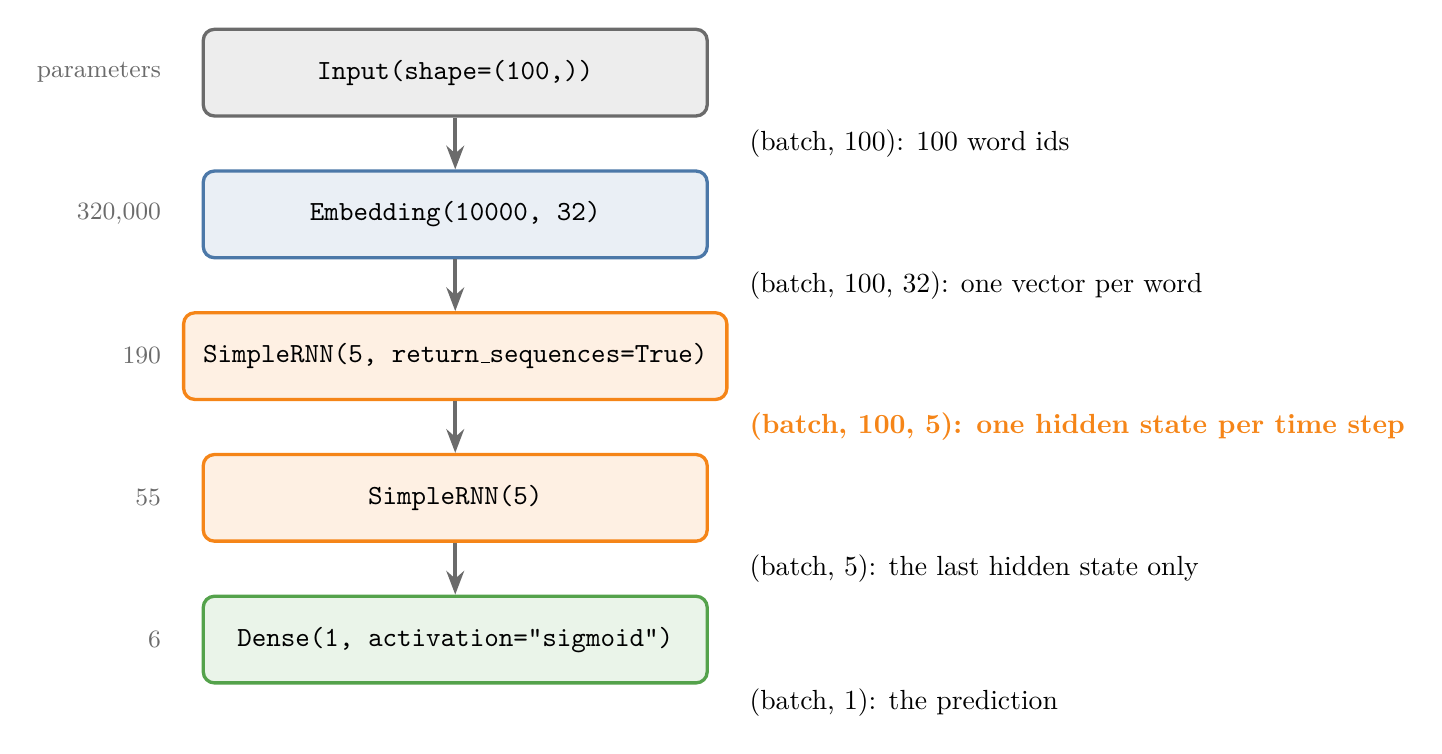
\begin{tikzpicture}[lay/.style={box=#1, minimum width=6.4cm, font=\sffamily}, sh/.style={font=\sffamily, anchor=west}]
  \node[lay=cgrey] (in) at (0,0) {\texttt{Input(shape=(100,))}};
  \node[lay=cblue] (emb) at (0,-1.8) {\texttt{Embedding(10000, 32)}};
  \node[lay=corange] (r1) at (0,-3.6) {\texttt{SimpleRNN(5, return\_sequences=True)}};
  \node[lay=corange] (r2) at (0,-5.4) {\texttt{SimpleRNN(5)}};
  \node[lay=cgreen] (d) at (0,-7.2) {\texttt{Dense(1, activation="sigmoid")}};
  \foreach \a/\b in {in/emb, emb/r1, r1/r2, r2/d} \draw[arrow] (\a) -- (\b);
  \node[sh] at (3.6,-0.9) {(batch, 100): 100 word ids};
  \node[sh] at (3.6,-2.7) {(batch, 100, 32): one vector per word};
  \node[sh, text=corange] at (3.6,-4.5) {\textbf{(batch, 100, 5): one hidden state per time step}};
  \node[sh] at (3.6,-6.3) {(batch, 5): the last hidden state only};
  \node[sh] at (3.6,-8.0) {(batch, 1): the prediction};
  \node[note, anchor=east] at (-3.6,-1.8) {320,000};
  \node[note, anchor=east] at (-3.6,-3.6) {190};
  \node[note, anchor=east] at (-3.6,-5.4) {55};
  \node[note, anchor=east] at (-3.6,-7.2) {6};
  \node[note, anchor=east] at (-3.6,0) {parameters};
\end{tikzpicture}
\end{document}
